\section{System Model}\label{sec_system}
The system model is composed of three parts: software applications, an execution platform, and an allocation scheme. In this section, we show models of the different parts and describe them detail. For smooth reading, first we list the main mathematical notations used throughout the paper, e.g., to define the system model and the software allocation problem.
\begin{table}[]
\begin{tabular}{@{}llp{0.65\textwidth}@{}}
\toprule
 & Notation                        & Description                                             \\ 
\midrule
$\bullet$ & \setExp{A}{A}     & a set of software applications, where $N-a=|A|$ \\
$\bullet$ & \sspExp{C}{i}     & a set of software component types, where $N_c=\abs{C}$ \\
$\bullet$ & \sssExp{Q}{q}    & a set of component replicas of type \sss{C}\\
$\bullet$ & \sssExp{R}[i]{r}[j]   & a set of runnables which implement \sss{C}\\
$\bullet$ & \sssxx{i}{T}{\tau}   & a set of runnables, where $N_\tau=\abs{T}$                \\
$\bullet$ &  \setExp{M}{m}         & a set of computation nodes, $N_m=\abs{M}$       \\
$\bullet$ & $\Gamma=\{\Gamma_i\ :i=1,\dots, N_\gamma\}$ & a set of end-to-end chains             \\
$\bullet$ & $\Gamma_i=(e_i)_{i=1}^Z$   & a chain of elements $e_i=r_i$ or $e_i=\tau_i$, $Z=\abs{\Gamma_i}$ is the length of the chain\\ 
$\bullet$ & $\zeta:T\mapsto R$ & a function that groups and maps runnables to tasks\\[6pt]

$\bullet$ & $c_{i,k}$                            & the component co-hosted at $A_k$         \\
$\bullet$ & $c_{ij,k}$                           & the $k^{th}$ replica of $c_{i,k}$        \\
$\bullet$ & $K_{i,k}$                            & the replica size of $c_{i,k}$\\[6pt]

$\bullet$ & $\textbf{x}:C\mapsto M$            & a feasible software allocation solution                  \\
$\bullet$ & $Power(\textbf{x})$                & total power consumption of applications $A$               \\
$\bullet$ & $Reliability_{i}(\textbf{x})$      & the reliability violation of application $A_i$              \\
$\bullet$ & $ResponseTime_{i}(\textbf{x})$     & the response time violation of task $A_i$                       \\
$\bullet$ & $Delay_{i}(\textbf{x})$            & the age delay violation of chains in $A_i$         \\
\bottomrule
\end{tabular}
\end{table}

\subsection{Software Applications}
The software applications are user-defined software systems, e.g., x-by-wire, electronic throttle control, flight control, etc., that are developed using software components \cite{softwarecomponents}\cite{Crnkovic2002BuildingSystems}. A software application $A_i$ is associated with high-level and user defined requirements $\langle RelReq_i, E2eReq_i,L_i\rangle$, where the tuple elements denote, respectively the reliabiity requirement, end-to-end timing requirements and criticality-level of the application $A_i$. The critical level signifies the importance of an application over other applications that have lower criticality levels, thus prioritizing the application during resource contention. The criticality levels are defined systematically, e.g., following the hazard analysis according to ISO 26262 standard. The end-to-end timing requirements define the timing constraints over end-to-end functional behaviors of applications, which are referred to as \textit{cause-effect chains}, and finally the reliability requirement defines the expected reliability goal of an application which is discussed further in Subsection \ref{subsec_reliability_constraint}. 

The software applications are run in parallel and therefore can potentially be distributed on different computation nodes $M =\{m_i:i=1,2,\dots J\}$, where $J=|M|$ is the total number of nodes, that we assume are heterogeneous with respect to processor speed, failure-rate and power consumption as indicated by the tuple $(hz, \lambda, p)$, respectively. 

%$\bigcup_{i=1}^{N_a} A_i$ 
\begin{definition}[Software Application Model]
It is modeled as \textit{undirected} graph $\langle V_c,L_c\rangle$ of software component nodes, where $a_{ij}\in L_c$ refers to the communication link from node $c_i$ to node $c_j$. It is associated to a function behavior that is modeled as \textit{directed acyclic vertex-weighted} graph $\langle V_\tau,L_\tau, w\rangle$ of periodic task nodes $V_\tau$, where $a_{ij}\in L_\tau$ refers to the data-flow link from node $\tau_i$ to node $\tau_i$ and $i \neq j$. The computation cost $w(\tau)=\langle e_m,D,P\rangle$ refers to the periodic task model of the node and the tuple elements denote the worst-case execution time {WCET} on node $m$, deadline and periodic activation, respectively.
\end{definition}

Multiple applications can be executed on the same computation node(s) and can share the CAN bus. Since the applications can have different criticality requirements, the execution platforms should provide a separation mechanism in order to avoid interference from lower-critical applications on higher-critical applications, e.g., fault propagation, also known as   \textit{mixed-critical} design \cite{Vestal2007PreemptiveAssurance}, which is an existing practice in avionics and also trending in other domains, e.g., automotive, where  safety-critical applications, such as x-by-wire and electronic throttle control systems, are required to be consolidated with the infotainment system on the same ECUs \cite{bibid}.

\subsection{Scheduling Software Applications}
The applications are scheduled on the execution platform by considering their respective requirements such as the criticality levels, reliability requirements, and end-to-end timing requirements. There are several techniques in the literature that deal with the scheduling of mixed-critical applications on a \textit{uniprocessor} systems \cite{Vestal2007PreemptiveAssurance}. In this work, we consider the \textit{partitioned criticality (PA)}  technique, which basically prioritizes higher critical applications over their lower critical counterparts. In contrast to other techniques, PA does not require a runtime monitoring of tasks, e.g., using servers \cite{AbeniIntegratingSystems,Ashjaei2017DesigningSystems,Inam2014ThePlatforms}.

\subsubsection{Scheduling Tasks}
By refinement, the tasks $Tasks_{A_i}$ and messages $Msg_{A_i}$ inherit the priority of $A_i$, essentially prioritizing higher critical tasks and messages, respectively at the computation and network levels \cite{Baruah2011Response-timeSystems,Burns2013MixedNetwork}. In this context, the task set allocated to node $m_i$, $T_{m_i}$ is scheduled by the \textit{fixed-priority preemptive scheduling polity} (FPPS), using the \textit{deadline monotonic} (DM) scheduler. The schedulability of the tasks is verified via the classical response time analysis (RTA) technique \cite{Baruah2011Response-timeSystems}. 

\subsubsection{Scheduling Messages on the CAN Bus}
Likewise, the messages in the CAN network bus are scheduled using fixed priority non-preemptive scheduling policy using.

\subsubsection{Scheduling Cause-effect Chains}

\subsection{AUTOSAR System}
The AUTOSAR standard introduced the notion of \textit{Runnables} to facilitate early analysis, that is at the VBF level, and to support interoperability of automotive applications across different execution platforms. Basically, runnables are schedulable piece of code similar to tasks. In this work, we assume periodically activated runnables with support for multiple worst-case executions that correspond to the different computation processor types. Unlike tasks, runnables' functional and extra-functional properties, e.g., timing, memory requirements, are part of the AUTOSAR software component specifications. Therefore, the software application model is extended to accommodate the notion of runnables, using the following simplified formal definition.

\begin{definition}[AUTOSAR Software Application Model]
It is modeled as directed acyclic vertex-weighted graph $g_r=\langle V_r, L_r, w, v\rangle$ of runnable nodes $V_r$, where $a_{ij}\in L_r$ represents either a triggering or data-flow link from the runnable $r_i$ to runnable $r_j$ and $i\neq j$. The cost at the node refers to the timing model of the runnable, where the tuple elements, respectively denote execution time on node $m$, deadline and period. 
\end{definition}

Essentially, the software applications are entirety developed using AUTOSAR software components, and eventually via as graphs of runnables. The refinement from a runnables graph to a tasks graph is conducted using the following heuristic rules, which is according to the AUTOSAR specification \cite{AUTOSAR2017SpecificationSoftware}. The rules are executed in order of appearance. Thus, the runnable link $(a, b)\in L_r$ merges to a task node $v\in V(g_r)$ if the following conditions hold':
% \begin{figure}[!h]
% \centering
% 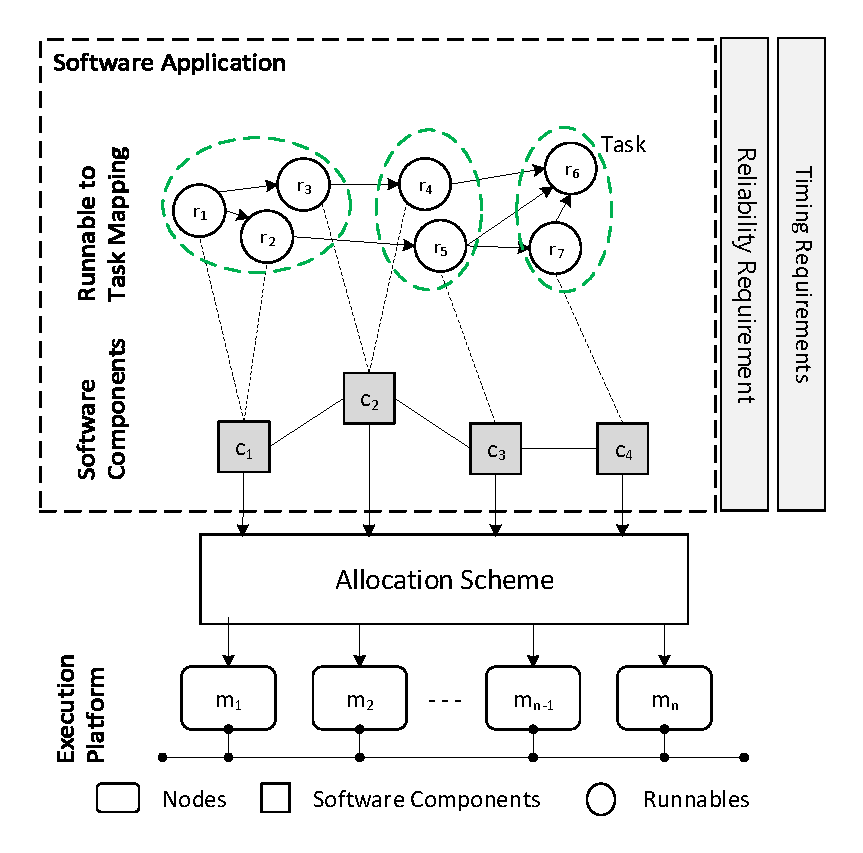
\includegraphics[scale=0.6]{softwareallocation}
% \caption{System Model.}
% \label{fig_softwareallocation}
% \end{figure}
\begin{description}
\item [Condition 1:] the runnables are co-hosted in the same computation node, i.e., \[a\mapsto m \land b\mapsto m\]
\item [Condition 2:] activation periods of the runnables are the same, i.e., $a.P = b.P$
\end{description}

If the condition hold, the task timing specifications are set as follows: i) the WCET of the task is set to the sum of the WCET of the runnables, i.e., $v.e_i=a.e_i + b.e_i$, ii) the period of the task is set to the period of the runnables, $v.P=a.P=b.P$. However, if condition 1 is satisfied but the runnables have different periods, the task period is set to the minimum of the runnables' periods, i.e., $v.P=Min(a.P, b.P)$. Otherwise, runnables are not merged, instead, each runnable is mapped to a task, while preserving the timing specifications.

% Following the grouping of runnables to tasks, We assume runnables communicate (or send data messages) at the end of the corresponding tasks' executions. The messages are packed into a single frame if destined to the same node otherwise each runnable communicats across a shared bus via a dedicated message entity, which is schedulable by the CAN bus controller. In essence, the assumed read-exec-write semantics of the runnables lowers the number of schedulable messages entities in the bus by facilitating packing of signals at the expense of restrictive (or less flexible) inter-runnables communication.

% Furthermore, we assume fixed and dynamic preemptive scheduling policies, that is each tasks sets allocated to a node must be schedulable according to the choice of the scheduling policy. For convenience, we assume priorities are assigned to tasks according to Rate Monotonic (RM) for the case of fixed scheduling policy, that is a task with a lower period get a higher priority.

\subsection{Execution Platform}
The execution platform provides computation and communication resources to the user applications, and is modeled as a \textit{complete} graph $\langle M,L^m\rangle$ of computation nodes, where $(m_i,m_j)\in L^m \land i\neq j$ refer to the communication links of the nodes, which are realized by a network bus, e.g., CAN. The computation nodes are heterogeneous with respect to parameters defined as a tuple $\langle hz, \lambda, p \rangle$, respectively denote processor speed, failure-rate and power consumption specifications. The allocation scheme is a mapping table $f:C\mapsto M$ from software components to computation nodes, where $C=\bigcup_{i=1}^{|A|} {V(A_i)}$ is the \textit{infinitary} union of the user applications' vertices, which denote nodes o software components.

\subsection{Fault-tolerant Software Application Model}
Redundancy is the most common way to increase the reliability of an application. It can be implemented according to different schemes, such as hot stand-by, cold stand-by, etc~\cite{Dubrova2013Fault-tolerantDesign}. In this work the details of the redundancy scheme are abstracted away under the following assumptions: i) Hot stand-by redundancy technique is used for the replacement of failed components, which are identical and are allocated on different nodes, ii) software components need to be replicated if the application's reliability requirement is not met without replication, otherwise they are not replicated, iii) the time needed to detect and replace a faulty component is considered negligible and will not be taken into account in the response time analysis of tasks and delay calculation of cause-effect chains, iv) Because of its simplicity, the mechanism for detection and replacement of faulty components will be considered fault-free, and therefore will not be included in the reliability calculations.

We denote the $k^{th}$ replica of a software component $c$ as $c^k$, with $1\le k\leq K$; where $K$ is the maximum number of replicas allowed for each application component.

%\subsection{Platform Model}
%The application is deployed on a network of heterogeneous computing nodes that are connected via a reliable communication network, the CAN bus. The computation node is specified as a 3-tuple $\langle hz, \lambda, p \rangle$, respectively, refer to the processor frequency, failure-rate and power consumption of a computation node. Due to the heterogeneity assumption of the processors, an application maybe be deployed on nodes with higher processor frequencies, and therefore fewer number of nodes in order to minimize the total power consumption of the system. However, due to the application reliability requirement, the application could be deployed differently, and with more resources. The CAN bus is considered reliable, for instance through redundancy. Therefore, its exclusion from the overall calculation of the system's reliability does not impact our proposed software allocation. %Figure~\ref{fig_softwareallocation} illustrates an overview of an AUTOSAR software application deployment on a set of computational nodes via a software allocation scheme that is discussed in Section~\ref{sec_allocation}.




%\subsection{AUTOSAR Software Application Model}
%AUTOSAR software applications are constructed from communicating AUTOSAR application components $\bigcup_{i=1}^{I} C_i$, where the component $c_i^k$ is the $k^{th}$ replica of the component type $C_i$ and $I$ is the number of software component types (or the cardinality of the infinitary union). Each software component co-hosts a set of runnables $R^*\subseteq R$ that are disjoint.
